\documentclass[crop,tikz,convert]{standalone}
\usetikzlibrary{shapes,matrix,positioning,chains,arrows,shadows,decorations.pathmorphing,fit,backgrounds}
\begin{document}

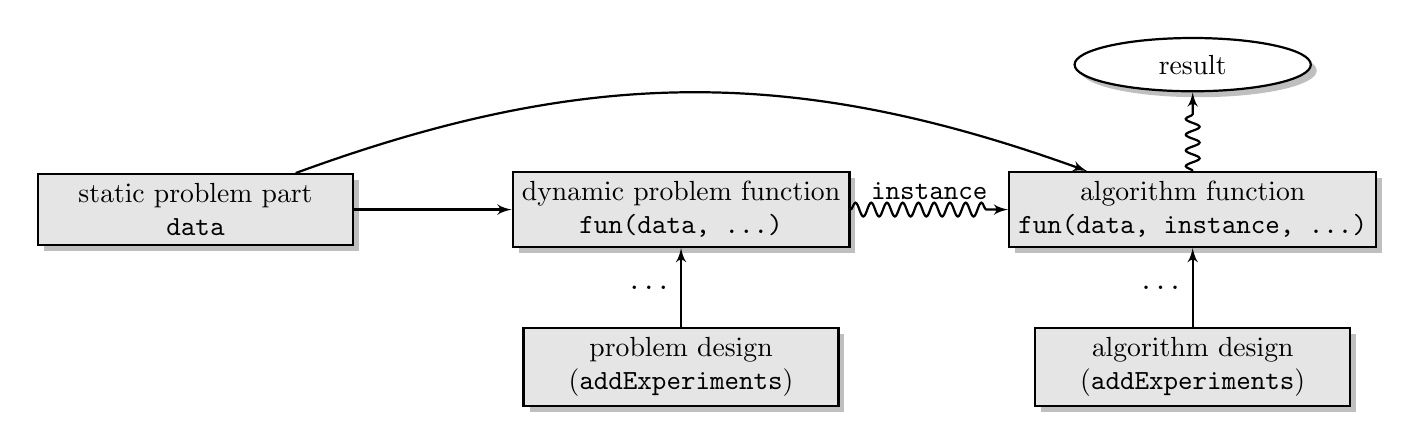
\begin{tikzpicture}[auto]
  \tikzstyle{userinput}=[rectangle, drop shadow, draw=black, fill=black!10, thick, minimum width=4cm, align=center]
  \tikzstyle{internal}=[rectangle, drop shadow, draw=black, fill=white, thick, minimum width=4cm, rounded corners, align=center]
  \tikzstyle{result}=[ellipse, drop shadow, draw=black, fill=white, thick, align=center, minimum width=3cm]
  \tikzstyle{line} = [draw, thick, -latex']
  \tikzstyle{sline} = [draw, thick, -latex',decorate, decoration={snake, segment length=2mm,post length=2mm}]

  \matrix [row sep=10mm, column sep=20mm] {
    % first row
    \node {}; &
    \node {}; &
    \node [result] (result) {result}; \\

    % second row
    \node [userinput] (static_problem_part) {
      static problem part\\\texttt{data}
    }; &
  \node [userinput] (dynamic_problem_part) {
    dynamic problem function\\
    \texttt{fun(data, ...)}
	}; &
	\node [userinput] (algorithm) {
    algorithm function\\
    \texttt{fun(data, instance, ...)}
	}; \\

	% third row
	\node {}; &
    \node [userinput] (problem_design) {
      problem design\\
      (\texttt{addExperiments})
    }; &
	\node [userinput] (algorithm_design) {
    algorithm design\\
    (\texttt{addExperiments})
	}; \\
  };

  \draw [sline] (algorithm) to (result) ;
  \draw [line] (static_problem_part) to (dynamic_problem_part);
  \draw [sline] (dynamic_problem_part) to node {\texttt{instance}} (algorithm) ;
  \draw [line] (static_problem_part) to [out=0, in=0, bend left=20] (algorithm);

  \draw [line] (problem_design) to node {\texttt{...}} (dynamic_problem_part);
  \draw [line] (algorithm_design) to node {\texttt{...}} (algorithm);
\end{tikzpicture}
\end{document}
